\chapter{Implementation}


\section{Hierarchy of Arrays}

The API of an array is defined by an interface called \textit{INDArray} which has a dense implementation for each backend: \textit{NDArray} class for the CPU and \textit{JCublasNDArray} class for the GPU. But since most of the operations and methods are shared between the two dense backends, they are implemented in an abstract class called \textit{BaseNDArray}.

Adding sparse representations asked two questions:
\begin{enumerate}
 	\item What can be shared with the dense arrays ?
	\item What can be shared between the different sparse arrays and what is format-specific ?
\end{enumerate}

To answer those questions, we need to go a little bit deeper in the implementation. 

The dense implementation includes methods that are inherently related to the way dense arrays are internally made, and other methods are related to the generic parameters such as the shape or are utility methods, and can be used independently of the internal implementation.

The first type of methods is not useful in case of sparse. Dense and sparse arrays are not built in the same manner. Methods such as \textit{getStrides} are not relevant in the sparse context. Reciprocally the sparse array will need methods which will be irrelevant in the dense context.

We encounter the same situation between the different sparse formats. Some will need utility methods that the other ones won't need.

However some methods should be reusable such as traversal operations which operate in an element-wise manner.

But as much as possible has to be exposed in the \textit{INDArray} interface. To avoid code duplication, everything than can be shared should be implemented in the higher level of the hierarchy. 

The methods that are not compatible with a type of array will simply throw an unsupported operation exception.

The drawback brought with this solution is that we always need to verify the type of the array before doing any operations.

// TODO update schema
 
\begin{figure}[H]
	\begin{center}
	%	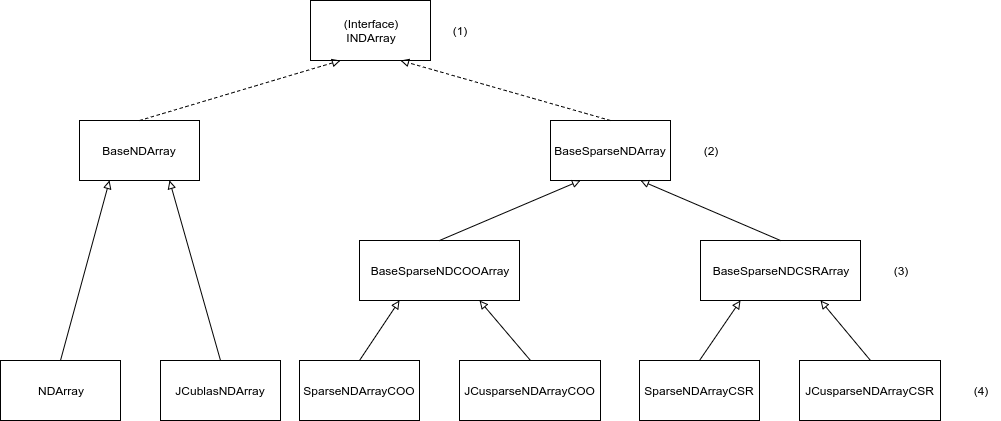
\includegraphics[width=6.5in]{images/INDArrayHierarchy.png} 
		\label{fig:hierarchy}
		\caption{Arrays hierarchy in Nd4j}
	\end{center}
\end{figure}


\section{Limitations and Constraints}

Nd4j has been made with the perspective of dense arrays. The design has been thought and optimized regarding the dense implementation which brings some constraints to implement the sparse representation
\subsection{Storing off-heap}

The data, encapsulated into DataBuffer object, is stored off-heap. Several reasons drive this design decision.
\begin{enumerate}
	\item The size of the memory that can be allocated within the JVM is limited to 2 billion. We can not fit some big matrices into the JVM.
	\item We want to use Cuda to accelerate the computation on the GPU. Cuda memory managment is not compatible with the JVM environment, the data has to be stored on the native side.
	
	In Cuda backend we store the data in a dual manner: one host copy (in the RAM) and one device copy on (on the GPU).
	
	\item Java execution is always sequential even with multi-threading, it cannot be parallelized on multiple CPUs. With C++ we can have cheaper parallel executions.
	\item At C++ level we can have easier access to SIMD (Single Instruction, Multiple Data) instructions that allow to execute an instruction in parallel on different blocks of the same data. Those instructions are heavily exploited by BLAS.
\end{enumerate}

\subsection{Workspaces}

The garbage collector makes the memory management of the JVM easier. It takes care of tracking the referenced object created by the program and remove them if there is no any longer reference pointing to the object. It automatically frees the unused allocated memory space. But the free operation is not immediate. The garbage collector has to pause the execution of the program at some point to modify the memory. Some unused memory spaces can still be temporarily allocated.

In machine learning and deep learning, many of the operations have a cyclic workload: we get a part of a dataset, we perform an operation and then we pass to the next data. Only the current values a relevant, the old memory content is not  used anymore. We want to avoid having too much previous data allocated.

Nd4j has implemented workspaces. A workspace is a memory chunk that we allocate once and which we can reused it as long as we need. The garbage collect does not manage this memory space. In a cyclic workload, we do not allocated a new memory space, we can use the space used by the last operation. The memory space size do not change, we only replace the content.



\subsection{DataBuffers have a fixed length}

Once allocated a \textit{DataBuffer} can not be reallocated. It is not a issue when manipulating dense arrays, we never need to add a new value in a dense array, we only update the existing values. However we need to be able to add new values in the sparse buffers. Each time a zero value become a non-zero value we have to put the value and its indexes in memory.

To reallocate a buffer we need to:
\begin{enumerate}
	\item Create a new \textit{Pointer} to a bigger memory space and replace the current pointer of the \textit{DataBuffer} .
	\item Create a new \textit{Indexer} with the new \textit{Pointer} and replace the current indexer of the \textit{DataBuffer}.
	\item Copy the content from the old \textit{Pointer} to the new space.
	\item The buffer has two length attributes: \textit{length} which count the number of values in the buffer and \textit{underlyingLength} which reflects the actual allocated size in memory. After the reallocation the \textit{underlyingLength} is increased to the new size, but the \textit{length} only increases at the insertion of a new value.
\end{enumerate}

We over-allocate the buffer in order to limit the amount of reallocation operations. Instead to expand the size to the new data length, we double the available memory space. The next time we want to insert some new values in the buffer, we avoid the expensive costs of the reallocation and the data copy.

Another possibility would have been to create a new \textit{DataBuffer} with the content of the old buffer plus the new value. But changing the DataBuffer object in a array would have broken the view mechanism since the views would still point to the old \textit{DataBuffer} reference. Moreover this solution doe not allow the over-allocation.


\section{CSR Matrices Implementation}

Nd4j does not provide any representation for this matrix format. We used the existing data structure, parameters holder and indexes to implement a new representation and the operations.

\subsection{Structure}

The representation uses 4 data buffers to encode a CSR matrix. One for the non-zero values, one for the columns indexes and two for the row pointers (to the beginning and to the end of each row).

\subsection{Put a value}

To insert a new value or to update an existing non-zero value, we need to identify where the values of row we want ot insert to are located in the values buffer and in the columns buffer. The beginning and end of rows pointers give us the range of indexes.

While iterating over the range of values, if we find a value with the same column index than the one we want to insert to, we can update the values and nothing needs to be changed in the three other buffers. 

However if there is no value with that column, we need to insert a new one at the correct position. Then we need to update the end of row pointer for this row. Finally each row pointers that come after need to be increment by one.

% TODO
-- ADD pseudo code for putscalar of csr? - coming soon!



\subsection{Get a Sub-array}

\begin{enumerate}
\item First, we need to compute the parameters such as the shape, the offsets,\dots of the sub-array. We use the \textit{ShapeOffsetResolution} which resolves a combination of indexes and returns the parameters. Despite this class has been made for resolving the indexes of a dense representation, we can reuse it in case of sparse array. The parameters we need are computed independently of the storage format and the internal structure of the array.

For example an interval $[1, 3[$ on a dimension $i$ would result to $offsets[i] = 1$ and $shape[i] = 2$, which is the length of the interval. It does not make any assumption about the underlying storage format.

Here are the parameters we need to compute:
\begin{itemize}
	\item the shape: an array with two elements containing the new shape of the sub-array.
	\item the offsets: an array with two elements that indicate the first row and the first column that belongs to the sub-array.
	\item the offset: indicates the position in the data buffer of the first element that belongs to the sub-array.
\end{itemize}
 \item Sometimes the offsets are equal to zeros while having a non-zero offset. This situation occurs for example when using only a combination of \textit{all} and \textit{point} indexes. In this case we need to compute the offsets manually.
  
 \begin{algorithm}
 	\caption{Calculate the offsets}
 	\label{alg:sparseOffsets2d}
 	\begin{algorithmic}
 		\Procedure{offsets}{int $offset$}\\
 		\Comment the shape array mentioned behind is the shape of the current array from which we are getting a view.
	 		\State $offsets \gets new\ int[2]$
	 		\State $offsets[0] \gets \lfloor offset\ /\ shape[1]\rfloor$
	 		\State $offsets[1] \gets offset\ \%\ shape[1]$
 		\EndProcedure
 	\end{algorithmic}
 \end{algorithm}
 
\item With the offsets and the shape we can define the bounds of each dimensions such has \\
$dim_{i} \in [offsets[i], offsets[i] + shape[i][$
\item Finally we need to loop over every element of the original array. We have to reconstruct the pointers buffers step-by-step by checking if the coordinates of the current element are included in the bounds and update the pointers buffers if needed.
\end{enumerate}

The entire method is shown in appendix \ref{lst:getcsc}.

\subsection{Limits of this format}

This format only works with two dimensions and cannot be extended to tensors. Therefore it makes it hardly compatible with the API.
Moreover the operations to get or put values aren't straightforward. Several step are necessary before accessing the value of a given coordinates:

Assuming we want to get the value $v_{i}$ of the coordinates $(r_{i}, c_{i})$.
 We have to get the two row pointers of $r_{i}$, iterate over the values buffer on the range delimited by the pointers and check if the column index of the current value is equal to the $c_{i}$. As soon as we match the column index, we can return the value $v_{i}$ or we return zero if we reach the end of the row without matching.

However we could use this format to represent Tensors Along Dimension (TADs) as explained in section \ref{sec:moreFormat}

\section{COO Tensors}

Conversely to the CSR format, the COO format can easily be extended to multi-dimensional array. Since we stored the coordinates of each value, the rank of the array is not limited to two, we can store any number of coordinates.
 
As the CSR representation, no implementation of a COO format exists in Nd4j, we have to create it using the existing components of the library.

\subsection{Naive implementation} \label{ssec:naiveCoo}

Based on the description in \ref{sssec:coo} the COO encoding needs one data buffer to store all the non-null values and one for the indexes of each values. 

An easy solution would have been to store the indexes into a multi-dimension array of \textit{DataBuffers}: One buffer for each value, or one buffer for each dimension. Due to the native constraints that makes hardly manageable to have such arrays (difficult to pass the array to the native side and Cuda side), we choose to flatten the indexes into one buffer.

The figure \ref{fig:datastoring} illustrates the different manner to store the coordinates $[0, 2, 1]$ of a value $v_{i}$ in a 3-order tensor with four non-zero values.

\begin{figure}[h]
	\centering
	\subfloat[each index is stored contiguously]{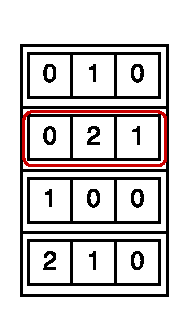
\includegraphics[width=1in]{images/indexesCoo_a.pdf} \label{fig:cooIdxA}}
	\quad
	\subfloat[Each dimension is stored contiguously]{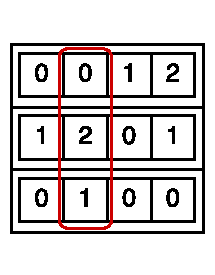
\includegraphics[width=1.1in]{images/indexesCoo_b.pdf} \label{fig:cooIdxB}}
	\quad
	\subfloat[Flattened Indexes]{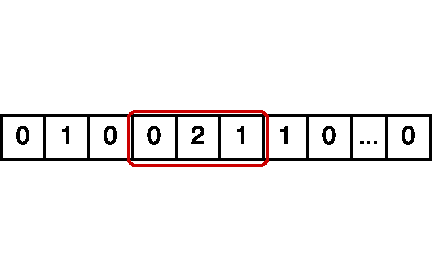
\includegraphics[width=2.3in]{images/indexesCoo_c.pdf} \label{fig:cooIdxC}}
	\hfill
	\caption{Illustration of the different possible data structure for storing the indexes  [0, 2, 1] of a value $v$ }
	\label{fig:datastoring}
\end{figure}


But this implementation makes difficult to be compatible with the API. It brings several issues:
\begin{itemize}
	\item The key of views is the sharing of their data to avoid the reallocation. In case of COO format, views have to share the data buffer and the indexes buffer. 
	We might be tempted to create an new indexes buffer for each view. Each indexes buffers will have the coordinates of the value regarding the view context. But it  would not be possible to add a value in the original array by adding it in a view. If we only put the new value in the shared value buffer without updating the indexes, the original array would have a value buffer bigger than its indexes buffer and we would not know what the indexes of this value are. 
	
	Even when sharing both buffers, how would we know which value is included in the view and which is not? 	
	
	\item The coordinates of a value in a view are not necessary the sames of the same value in the original array. 
		
	They can be offset if dimension is partially included in the view. Figure \ref{fig:viewOffset} shows a matrix an a view (in red). The value$ v_{i}=5$ would have the coordinates [1, 1] in the original array while it has the coordinates [0, 0] in the view. How can the indexes be translated between views?
	\begin{figure}[!h]
		\centering
		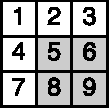
\includegraphics[width=0.8in]{images/viewIndexOffset.pdf}
		\caption{A $3\times 3$ matrix with a $2\times 2$ view in grey}
		\label{fig:viewOffset}
	\end{figure}

	\item A view can have a lower or higher rank than its original array. How can the view indexes be stored if they do not have the same dimensionality?
\end{itemize}

\subsection{Reverse coordinates}
\label{ssec:reverse}
An important and frequently used method of the API is to get the value of a set of coordinates. Since the indexes are flattened into one buffer, we need to find them into  the buffer and get the underlying index and then the corresponding value.

Since the indexes buffer is lexicographically sorted, a binary search can be applied. But instead of comparing a value, we need to compare a sub-array of the buffer with the target indexes. An additional step is necessary before the comparison: translate the position of the value in the values buffer to get the positions of the indexes in the buffer.

We iterate over the values (NNZ elements) and for each value $v_{i}$, we extract the sub-array that contains the coordinates of $v_{i}$

The subarray of a value $v_{i}$ is contained between the following indexes: 
\begin{lstlisting}[style=nonumbers]
	idx_from = underlyingRank * i;
	idx_end = idx_from + underlyingRank;
\end{lstlisting}

The underlyingRank is the number of coordinates used to index a single value in the original array buffer.



\subsection{Put a Value}

Several steps are needed to put a new value in a COO array:
\begin{enumerate}
	\item The same value in a view or in the original array can have different coordinates. A translation step is needed between the view indexes and the original array coordinates (the actual coordinates stored in the shared buffer).
	\item Verify if the old value of this index is already non-zero. If so we can either remove the entry if the new value is zero, or replace the old value by the new in the buffer. Nothing else need to be done.
	\item If the new value is equal to 0: the indexes and the value are not added in the buffers.
	\item If it is a new non-zero value: we need to insert the value and the indexes in the buffers. But first we need to ensure that the buffers have enough spaces for the new entries. If not, we need to reallocate them. The new entries are added at the end of the buffers; the sort are not maintained at insertion to avoid sorting the array too often when it is not needed. 
	
	For example an operation that modifies sequentially the values (i.e traversal operation) might need to add multiple non-zero values in memory. If the sort was maintained at insertion, we would need to pay the cost of searching the right position for each value. 
\end{enumerate}


\subsection{More parameters are needed to define the tensors}

Nd4j uses a powerful tool to access part of an array: the \textit{INDArrayIndexes}. But they are the sources of many of the issues cited in section \ref{ssec:naiveCoo}.

We present each type of index, with their set of constraints and the solutions implemented below.

\subsubsection{Resolution of the Indexes}

The \textit{ShapeOffsetResolution} is a key mechanism in the resolution of the indexes. Taking a combination in input, it computes the information such as the shape, the offsets, the strides,\dots about the sub-array selected by the indexes. 

Despite this class has been made for resolving the indexes of a dense representation, we can reuse with sparse arrays. The parameters we need are computed independently of the storage format and the internal structure of the array.

For example an interval [1, 3[ on a dimension i would result to $offsets[i] = 1$ and $shape[i] = 2$, which is the length of the interval. It does not make any assumption about the underlying storage format.

\subsubsection{All Indexes}
\textit{All} indexes are the most straightforward of the library. They are used to collect all the elements of a dimension. They are useful when used in combination with other type of indexes. For example if we would like to take the first column of a matrix, we would need to ask for the first element of all the rows.

\subsubsection{Interval Indexes}
\textit{Interval} indexes takes an contiguous subpart of a dimension containing in an interval. They don't modify the rank

The grey sub-array in figure \ref{fig:viewOffsetDup} is the result of the operation :
\begin{lstlisting}[style=nonumbers]
	myArray.get(NDArrayIndex.interval(1, 3), NDArrayIndex.interval(1, 3));
\end{lstlisting} 

\begin{figure}[!h]
	\centering
	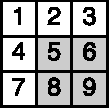
\includegraphics[width=0.8in]{images/viewIndexOffset.pdf}
	\caption{A $3\times 3$ matrix with a $2\times 2$ view in grey}
	\label{fig:viewOffsetDup}
\end{figure}

After the resolution of the indexes, we obtain offsets equal to $[1, 1]$ with an offset equal to $4$, which mean that the first row and the first column are not included in the view and the first element in memory that belongs to the view is at position $4$ in the original array (the value 5 in the figure).

To be able to identify what values belong to the view and what values do not, we need to define the bounds of each dimension. For this example, we have

$(idx_{row}, idx_{colum}) \in view $  if  $idx_{row} \in [1, 3[$ and $idx_{column} \in [1, 3[$

We only need to store the lower bound $i_{lower}$ of the interval $idx_{dim} \in [i_{lower}, i_{upper}[$, we can easily compute $i_{upper} = i_{lower}+shape[dim]$.
The lower bounds are stored in the \textit{sparseOffset} array.

\subsubsection{Point Index}
\textit{Point} indexes take one unique element of a dimension. They reduce the rank of the array.

Assuming we have a tensor with a shape equal to ($2\times 3\times 3$) as shown in figure \ref{fig:pointTensor}. We want to take a slice along the first dimension, assuming that the first dimension is called the pages, the second the rows and the third the columns. We use the following operation to get the first page:
\begin{lstlisting}[style=nonumbers]
	myTensor.get(NDArrayIndex.point(0),
		NDArrayIndex.all(),
		NDArrayIndex.all());
\end{lstlisting} 

The result is a view with a shape equals to ($3\times 3$), as shown in grey in figure \ref{fig:pointTensor}

\begin{figure}[!h]
	\centering
	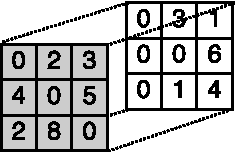
\includegraphics[width=1.5in]{images/tensorsHiglighted.pdf}
	\caption{A $2\times 3\times 3$ tensor with a slice along the first dimension in grey}
	\label{fig:pointTensor}
\end{figure}

The coordinates of the resulting matrix have only two dimensions instead of three. We have an issue when trying to access a value given a pair of coordinates in the view context. There is no direct matching between these coordinates and those who actually are in the indexes buffer. 

In the example above, the indexes buffer is equal to $[0, 0, 1, 0, 0, 2, 0, 1, 0, \dots]$ which correspond to the values buffer $[2, 3, 4, \dots]$.
The value $4$ has the coordinates $(0, 1, 0)$ while its coordinates in the view are equal to $(0, 1)$.

Generalizing, each value of the tensor has its coordinates in the form $(idx_{0}, idx_{1}, idx_{2})$. But in the resulting view the values are defined with only two coordinates: ($idx_{1}, idx_{2}$), the first dimension is fixed with a value equal to 0. 

To translate the view coordinates to the original coordinates which are actually stored into the shared buffer, we need to keep track of the unused dimension and its value. The solution is to add an additional parameter array that keeps track of the status of each dimension. The array is called \textit{flags} and it can contains either 0, which means \textit{active}, or 1 which means \textit{fixed}.

In this example the flags array would be equal to [1, 0, 0] because the first dimension is fixed at position 0. The value 0 would be keep into the \textit{sparseOffset} array. And the indexes translation would be : T($idx_{1}, idx_{2}$) = ($sparseOffset[0], idx_{1}, idx_{2}$)


\subsubsection{Specified Index}

Specified index will take non-contiguous values of a dimension, depending on the position in the indexes array when calling $myArray.get(indexes...)$. This index takes an array as argument containing the values we want to select.

Assuming we have an $3\times 5$ matrix, as shown in figure \ref{fig:specifiedArray}, on which we call the following operation to select the first, the third and the fourth columns :

\begin{lstlisting}[style=nonumbers]
	myMatrix.get(NDArrayIndex.all(),
		new SpecifiedIndex(0, 2, 3));
\end{lstlisting}

Instead of returning a view of $myMatrix$, it returns a new array containing the data from the original matrix. The data is copied, not shared. The data of the view that would result from this operation is not easily indexable in memory with stride and offsets and it would be difficult to represent it. Therefore the figure \ref{fig:specifiedCopy} is an independent $3\times 3$ matrix resulting from the above operation.

\begin{figure}[!h]
	\centering
	\subfloat[A $3 \times 5$ matrix with selected columns in grey]{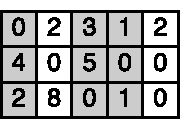
\includegraphics[height=1in]{images/specifiedIndex.pdf} \label{fig:specifiedArray}}
	\qquad
	\subfloat[A $2\times 2$ matrix created from the column of the matrix in figure \ref{fig:specifiedArray} ]{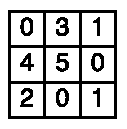
\includegraphics[height=1in]{images/specifiedIndexView.pdf} \label{fig:specifiedCopy}}
	\hfill
	\caption{Example of a specified index behavior on a matrix}
\end{figure}


\subsubsection{New Axis Index}
\textit{New axis} indexes are used to add a new dimension to the array. The new dimension always has a length equal to 1. It can be prepended or inserted in the middle of the dimensions.
Since the rank is higher, more coordinates are needed to access a value. However the shared indexes buffer is limited to the original rank. Similarly to the point index, we need a new parameter array that keep tracks of the position of the new dimensions to be able to translate the coordinates from view to original context.

Assuming we have a $3\times 3$ matrix: calling \textit{myArray.get(NDArrayIndex.newAxis(), NDArrayIndex.all())} will prepend a new dimension. The view is a $1\times 3\times 3$ tensor with a hidden dimension parameter array equal to $[0]$.

We use an array called \textit{hiddenDimension} to keep track of the position of the new dimensions in the coordinates. In the example above, each value $v_{i}$ has the coordinates $(i_{0}, i_{1}, i_{2})$ within the view context. The array \textit{hiddenDimension} contain $[0]$ because this dimension does not exist in the original array.

\subsection{Sparse Indexes Translation}
\label{ssec:translation}

To translate a view coordinates to the underlying coordinates, we have to take into accounts: the sparse offsets, the hidden dimensions and the flags. With those three parameters we have everything needed for translating.



While iterating over the view dimensions, three situations can happen :
\begin{enumerate}
	\item The current dimension is hidden; the original array does not contain it becaise it has been created by a \textit{point} index: We do nothing. The dimension is skipped and we start the next iteration.
	\item The current dimension is fixed: We put the corresponding offset into the result array. Since several fixed dimensions can occur one after the others in the coordinates array, we need to repeat until we reach an active dimension.
	\item The current dimension is active: We sum the view coordinate with the sparse offset.
\end{enumerate}
This method is described in detail in algorithm \ref{alg:translation} 


\begin{algorithm}
	\caption{Translate the indexes from view to underlying context}
	\label{alg:translation}
	\begin{algorithmic}
		
		\Procedure{translate}{int[] $viewIndexes$}\\
		\Comment{ $underlyingRank$ is the rank of the original array which is equal to the number of indexes stored in the buffer for a given value. 
		$hiddenDimensions$ contains the position of each hidden dimension.
		$sparseOffsets$ contains the offsets for each dimension. They are class fields of the COO array instance.}\\
		\State $result \gets new\ int[underlyingRank]$
		\State $idxPhy \gets 0$ \\ 
		\State $hidden \gets 0$ \Comment{Number of hidden dimension encountered}
		\\
		\For{$idxVir=0$ to $viewIndexes.length$}\\
		
		\Comment{The current dimension is hidden, it does not appear in the result}
		\If{$hidden < hiddenDimension.length \And hiddenDimension[hidden] == idxVir$}
		\State $hidden \gets hidden + 1$
		\Else
		\While{$idxPhy < underlyingRank \And isFixed(idxPhy)$}
		\State $result[idxPhy] \gets sparseOffsets[idxPhy]$ \Comment{If the dimension is fixed, the coordinate takes the value of the offset}
		\State $idxPhy \gets idxPhy + 1$
		\EndWhile\\
		\Comment{If the dimension is not fixed, we add the offset to the coordinate}				
		
		\If{$idxPhy < underlyingRank \And  !isFixed(idxPhy)$}
		\State $result[idxPhy] \gets sparseOffsets[idxPhy] + viewIndexes[idxVir]$ 
		\State $idxPhy \gets idxPhy + 1$
		\EndIf
		
		\EndIf
		
		\EndFor	
		\Return $result$ \Comment{contains the indexes of the underlying array}	
		\EndProcedure
	\end{algorithmic}
\end{algorithm}
\subsubsection{Example of indexes translation}

An example of execution is explained in appendix \ref{ssec:idxtrans}.

\subsection{Computations of the the Parameters}
\subsubsection{Computation of the Sparse Offsets}
\label{sssec:sparseOff}
The \textit{sparse offsets} are computed from the offset resulting from the resolution of the indexes. The \textit{offset} gives us the position of the first element in the array. 


\begin{enumerate}
	\item For each dimension except the innermost one, we divide the offset by the length of that dimension. The quotient gives us the sparse offset for the dimension. Then we need to remove the number of elements that are in the same dimension but at a lowest value (if the element is in the 4th row, we want to remove all the elements of the previous rows).
	
	\item We reached the last dimension: To compute the sparse offset of the last dimension we need to take the modulo of the updated offset by length of the dimension. 
	
	In steps 1 and 2 there is only one operation to compute the sparse offset per dimension, then for a n-order tensor, the complexity of these steps is O(n).
	
	\item We have the sparse offsets given a set of indexes. But if we are computing the sparse offsets of a view of a view, the view from which we are taking a view might already have some sparse offsets. We need to merge the new sparse offsets with those of the current array. The final result is the sum of the existing offset and the freshly computed offset.
		
	During the merge we should be particularly careful with fixed dimensions of the current array because they are absent from the sparse offset resolution explained above. The result does not contain any information about them, we need to add these fixed dimensions at the correct position with their current sparse offset to final offsets array. 

\end{enumerate}

\begin{algorithm}
	\caption{Calculate the sparse offsets}
	\label{alg:sparseOffsets}
\begin{algorithmic}
	\Statex
	\Procedure{CreateSparseOffsets}{int $offset$}\\
	\Comment{$rank$, $underlyingRank$ (the rank of the original array and the number of dimension of the indexes buffer), $shape$ and $sparseOffsets$ are class fields of the array instance}\\
	\State $newOffsets\gets new\ int[rank]$ \Comment{Compute the new offsets}
	
	\For{$i=0$ to $(rank - 2)$} 
	\State $nbElements \gets \prod_{j=i+1}^{rank} shape[j]$
	\State $newOffsets[i] \gets \lfloor offset \div nbElements\rfloor$
	\State $offset \gets offset - newOffsets[i] \times nbElements$
	\EndFor
	\State $newOffsets[rank-1] \gets offset \mod shape[rank-1]$ 
	\\
	\\	
	\State $finalOffsets\gets new\ int[underlyingRank]$	\Comment{Merge with sparseOffsets of this array}
	\State $active\gets 0$
	\For{$i=0$ to $underlyingRanke$}
	\If {$flags[i] == 0$} \Comment{If the dimension is already inactive in the current array}
	\State $finalOffsets[i] \gets sparseOffsets[i]$
	\Else
	\State $finalOffsets[i] \gets newOffsets[active] + sparseOffsets[i]$
	\State $i \gets i + 1$
	\EndIf
	\EndFor
	\Return $finalOffsets$
\EndProcedure
\end{algorithmic}
\end{algorithm}

\subsubsection{Example of Sparse Offsets Computation}
An example of the execution of the algorithm is presented in appendix \ref{ch:spaoffexec}

\subsubsection{Computation of the Flags}
The \textit{Flags} array determines which dimension is active and which one is hidden from the point of view of the array. The \textbf{}dimension can only be reduced using a \textit{point} index, which means the flags can be computed during the offset resolution. An \textit{interval} with a length equals 1 does not reduce the dimensionality of the array. We fill the flags array while iterating over the indexes array.

\subsubsection{Computation of the Hidden Dimensions}

The resolution returns an array containing the position of the \textit{newAxis} indexes in the indexes array. The array may already have some hidden dimensions. In this case we need to adapt the result with the current hidden dimension.

\begin{algorithm}
	\caption{Calculate the hidden dimensions}
	\label{alg:hiddenDim}
	\begin{algorithmic}
			
		\Procedure{CreateHiddenDimensions}{int[] $newAxis$}\\
		\Comment{$hiddenDimensions$ is a class field of the array}\\
		
		\If {$newAxis$ is empty or null}
		\Return {$hiddenDimensions$}		
		\EndIf
		\\
		\If {$hiddenDimensions$ is empty}
		\Return {$newAxis$}		
		\EndIf
		\\	
		
	
		\State $size\gets newAxis.length + hiddenDimensions.length$ 	\Comment{Merge both arrays}
		\State $newArray \gets $ new $int[size],\ newArrayIdx\gets 0,\ newDim\gets 0$
		\\
		\For{$(oldDim=0$ to $hiddenDimensions.length)$}
			\While{$((oldDim \geq hiddenDimensions.length \parallel newAxis[newDim] \leq hiddenDimensions[i])\ \&\&\ newDim < newAxis.length)$}
				\State $newArray[i] \gets newAxis[newDim] + oldDim$
				\State $newArrayIdx \gets newArrayIdx + 1 $
				\State $newDim \gets newDim + 1$	
			\EndWhile
			\State $newArray[i] \gets hiddenDimensions[oldDim] + newDim$	
			\State $newArrayIdx\gets newArrayIdx + 1$
		\EndFor
		\Return{$newArray$}
		\EndProcedure
	\end{algorithmic}
\end{algorithm}






\subsection{Final Implementation}
	
	The final representation is encoded with 5 \textit{DataBuffers}:
	\begin{enumerate}
		\item Values: Store the values linearly.
		\item Indexes: Store the flattened indexes of each values.
		\item Flags: Define which dimensions are active and which are fixed.
		\item Sparse Offsets: Define the bounds of each dimension.
		\item Hidden Dimensions: Keep track of the position of the hidden dimension in the shape array .
	\end{enumerate}
	
		The indexes and values are sorted in the lexicographic order in order to make the search by indexes easily via binary search. We sort the buffers only before we need to read them : when performing an operation or when accessing its contents. The sort is not maintained at the insertion.
		
		The flags, the offsets and the hidden dimensions arrays are grouped in one \textit{DataBuffer}, similarly to the \textit{ShapeInformation} buffer.
		
\subsubsection{Example}
Figure \ref{fig:tens} shows a tensor $T$ with a shape $(2\times 3\times 3)$ and Figure \ref{fig:tensView} shows the view resulting from the operation below:

\begin{lstlisting}
	T_view = T.get(NDArrayIndex.newAxis(), 
		NDArrayIndex.point(0),
		NDArrayIndex.interval(1, 3), 
		NDArrayIndex.interval(1, 3));
\end{lstlisting}

The first index prepends a new dimension and increases the rank, the second takes the first page of the tensor and reduces the rank. Then the next ones select the sub-array in the first page dimension. The parameters of $T_{view}$ are listed in figure \ref{eqn:viewParams} 

\begin{figure}[!h]
	\centering
	\subfloat[A tensor $T$ with shape $(2\times 3\times 3)$ ]{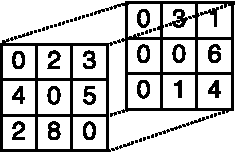
\includegraphics[width=1.7in]{images/tensors.pdf} \label{fig:tens}}
	\qquad
	\qquad
	\subfloat[A view of tensor $T$ with shape $(1\times 2\times 2)$]{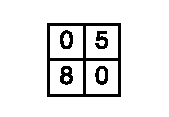
\includegraphics{images/tensors-view.pdf} \label{fig:tensView}}


	\caption{A tensor and a view of it }
	\label{fig:example}
\end{figure}
	
\begin{figure}[!h]

		\[
		\begin{aligned}
		Shape = 
		\begin{bmatrix}
		1 & 2 & 2 
		\end{bmatrix}
		\quad
		Values = 
		\begin{bmatrix}
		5 & 8 
		\end{bmatrix}\\			
		Indexes = 
		\begin{bmatrix}
		0 &  1 & 2 & 0 & 2 & 1
		\end{bmatrix}		
		\quad	
		Flags = 
		\begin{bmatrix}
		1 & 0 & 0
		\end{bmatrix}\\			
		SparseOffsets = 
		\begin{bmatrix}
		0 &  1 & 1
		\end{bmatrix}
		\quad		
		HiddenDimension = 
		\begin{bmatrix}
		0 
		\end{bmatrix}\\	
		\quad	
		\quad	
		\\
		Values = 
		\begin{bmatrix}
		2 & 3 & 4 & 5 & 2 & 8 & 3 & \dots & 4
		\end{bmatrix}\\			
		Indexes = 
		\begin{bmatrix}
		0 & 0 & 1 & 0 & 0 & 2 & 0 & \dots & 2
		\end{bmatrix}\\			
		\end{aligned}
		\]
		\caption{Parameters defining the view $T_{view}$ in \ref{fig:tensView}}
		\label{eqn:viewParams}
\end{figure}

\subsection{Get a Sub-Array}

The new parameters make the task easier. Once the indexes resolved and the parameters computed, a new array is created with the current values and indexes buffers and the new parameters. 

However if one of the indexes is a \textit{SpecifiedIndex} we need to create a new array and copy the data. In this case the index resolution translates any type of indexes to a specified index:

Assuming we have a $3 \times 3 \times 3  \times 3$ 4-order tensor. The indexes array of the following operation:
\begin{lstlisting}[style=nonumbers]
	myTensor.get(NDArrayIndex.all(),
		NDArrayIndex.point(1),
		NDArrayIndex.interval(0, 2),
		new SpecifiedIndex(0,2));
\end{lstlisting}
  would become : [SpecifiedIndex(0,1,2), SpecifiedIndex(1), SpecifiedIndex(0,1), SpecifiedIndex(0,2)]. 

Then we iterate over all the included combinations of coordinates and add the elements into a new empty array.

